\section{A Block Successive Over Relaxation Method}
\label{sec:block_sor}

Applying the correlation operator described in this paper, $\corrMat^{1/2}$,
requires the solution to an elliptic equation.
Here we describe the block-Successive Over Relaxation (SOR) method that was
implemented to solve this problem.
We note that both preconditioned conjugate gradient algorithms exist in the
MITgcm for 2D (in the latitude longitude plane) and 3D fields.
However, the preconditioner for these solvers is designed specifically for the
pressure solve at each time step \citep{marshall_finite-volume_1997},
and so may not be generally applicable to our problem.
As such, we opted to implement the SOR algorithm outlined here because it was
simple to do so, and efficient enough for our purposes.

The SOR method is an iterative method for solving $\mathbf{A}\mathbf{x} = \mathbf{b}$.
At iteration $k$, the elements of $\mathbf{x}$ are $x_i^k$, and we seek the update:
\begin{linenomath*}\begin{equation}
    \tilde{x}_i^{k+1} = (1-\omega) x_i^k + \dfrac{\omega}{a_{ii}}
    \left( b_i - \sum_{j<i}a_{ij}\tilde{x}_j^{k+1} -
        \sum_{j>i}a_{ij}x_j^{k}\right), \qquad
        i=1,2,...,N \, ,
    \label{eq:sor_update}
\end{equation}\end{linenomath*}
where the elements of $\mathbf{x}$ are $x_i^k$ (and similarly for $\mathbf{A}$
and $\mathbf{b}$), and $\omega$ is the SOR parameter.
Here the notation $\tilde{x}_i^{k+1}$ refers to the fact this is a local update,
i.e. there is no communication between the processes assigned to each portion of
the computational domain.
The only areas where this local update causes the algorithm to deviate from a
standard SOR method is when neighboring elements
$\tilde{x}^{k+1}_{j}, i\ne j$ are in the ``halo'' regions of a process's
subdomain which are only updated at the end of each iteration.
In this case, these neighboring elements take on the value from the previous
iteration: $\tilde{x}^{k+1}_j = x^k_j$.

\begin{figure}
    \centering
    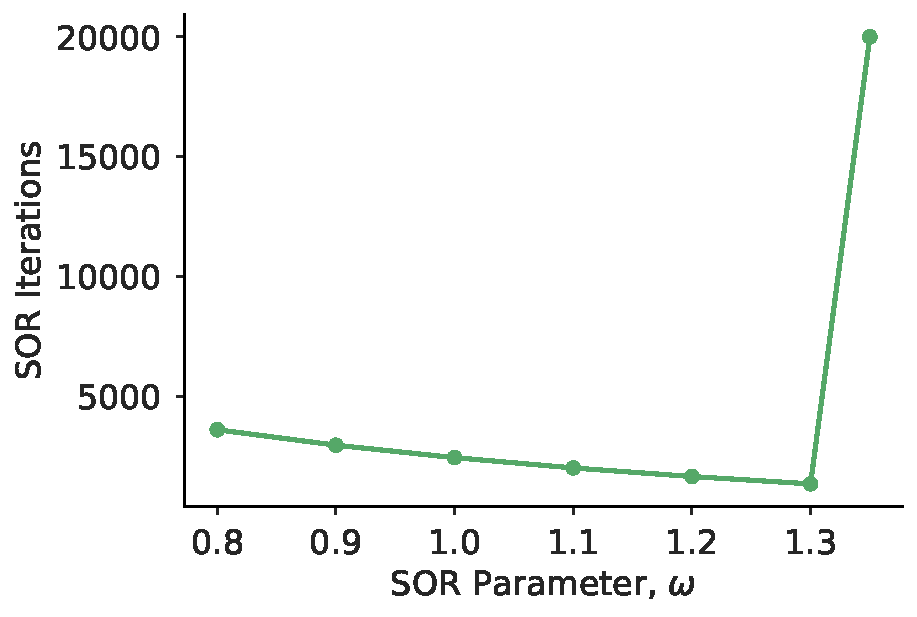
\includegraphics[width=.5\textwidth]{../figures/smith_fig8.pdf}
    \caption{Performance of the SOR algorithm for various settings of $\omega$
        using 10 samples, $\rangeh=10$, tolerance of $10^{-15}$, and $M=1$.
    }
    \label{fig:sor}
\end{figure}

We find this simple implementation to be an effective method for solving the
linear system.
\cref{fig:sor} shows the number of iterations required for
convergence as a function of the parameter $\omega$, with an optimal value of
approximately $\omega^*=1.3$.
We note that the number of iterations required to converge at this optimal value
is about half that of $\omega=1$, which coincides with a (block) Gauss-Seidel algorithm
(again differing from it's true form due to the halo updates).
Of course, \cref{fig:sor} shows the major drawback of the SOR algorithm: near
the ``optimal'' value for the SOR parameter, efficiency is highly sensitive.
For our implementation, at $\omega=1.35$, we see that the algorithm does not
fully converge and runs until set limit of 20,000 iterations.
